\chapter{Analisi}
L'attività di analisi iniziale, ovvero senza l'ausilio di librerie specifiche per l'invio di determinati pacchetti, è stata effettuata installando un Server Apache sia su Windows 11 che su sistema operativo Kali.
Si è quindi proceduto ad inviare richieste ai server tramite browser web e all'analisi dei pacchetti ricevuti in risposta con l'utilizzo di Wireshark.
Successivamente sono state analizzate anche le risposte a determinati pacchetti inviati con Scapy.
Di seguito sono riportate le differenze più importanti rilevate durante l'intera attività di analisi.
\section{Analisi a livello 2}


\section{Livello 3: protocolli IP e ICMP}
È stata effettuata in primis l'analisi del TTL (\textit{Time To Live}), essendo un valore estremamente semplice da analizzare.
Questo campo contiene un numero intero positivo che viene decrementato ad ogni \textit{hop}, ovvero ad ogni router che il pacchetto incontra nel percorso verso l'host ricevente, e viene eliminato dalla rete quando questo raggiunge lo 0.
Il protocollo, però, non impone nessun valore di partenza, lasciando libertà di scelta al sistema operativo del mittente; l'unico limite è rappresentato dagli 8 bit riservati a quel campo (ovvero ad un valore massimo di 255).
L'analisi ha portato ad evidenziare la seguente differenza riguardo al TTL:
\begin{table}[H]
	\centering
	\begin{tabular}{ l | c }
		\hline
		\rowcolor{blue!10} Windows 11 & 128
		\\
		\hline
		\rowcolor{red!10} Kali & 7
		\\
		\hline
		
	\end{tabular}
	\caption{TTL iniziale}
	\label{tab:TTL}
\end{table}

È inoltre stata effettuata l'analisi del protocollo ICMP, e in particolare è stata notata una differenza nel campo \textit{code} in caso di risposta a determinati pacchetti inviati utilizzando la libreria di Python scapy.
\\

\begin{figure}[H]
	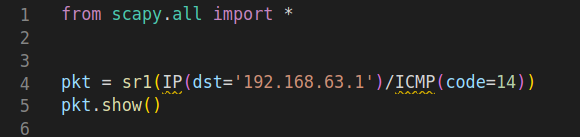
\includegraphics[width=\textwidth]{figures/icmp.png}
	\caption{Comando python per l'invio del pacchetto specifico}
	\label{congestione}
\end{figure}

Questo comando invia un pacchetto ICMP con il campo \textit{code} impostato ad un numero casuale, in questo caso 14: in questo specifico contesto, Windows 11 risponde inviando un pacchetto in cui \textit{code}=0, mentre Kali copia il valore che ha ricevuto nella richiesta.

\begin{table}[h]
	\centering
	\begin{tabular}{  l | c }
		\hline
		\rowcolor{blue!10} Windows 11 & 0
		\\
		\hline
		\rowcolor{red!10} Kali & Stesso valore inviato nella richiesta
		\\
		\hline

	\end{tabular}
	\caption{Campo code quando nella richiesta è diverso da 0}
	\label{tab:code}
\end{table}

\section{Livello 4: analisi protocollo TCP}
Il livello 4 dello stack è formato da due protocolli: User Datagram Protocol (UDP) e Transmission Control Protocol (TCP). Entrambi forniscono informazioni utili per il fingerprinting, ma il TCP possiede un numero maggiore di campi e di opzioni utilizzabili, pertanto è stata data priorità all'analisi di quest'ultimo.

Analizzando l'handshake TCP, si può notare una discrepanza nell'utilizzo del Window Scale; quest'opzione consente di aumentare la Window Size oltre il valore che si otterrebbe settando tutti i bit di quel campo a 1.
Ciò è dovuto al fatto che il valore dell'opzione rappresenta il numero di shift verso sinistra dei bit del Window Size, che corrispondono a raddoppi del valore contenuto. 
L'utilizzo di questa opzione viene concordato nei segmenti SYN e SYN+ACK dell'handshake e il suo valore non viene più modificato per il resto della connessione. Confrontando i valori ottenuti da Windows 11 e Kali, si ottiene il seguente risultato:
\\
\begin{table}[htb]
	\centering
	\begin{tabular}{ l | c }
		\hline
		\rowcolor{blue!10} Windows 11 & 8
		\\
		\hline
		\rowcolor{red!10} Kali & 7
		\\
		\hline
		
	\end{tabular}
	\caption{Window Scaling Factor}
	\label{tab:Window Scale}
\end{table}

Proseguendo l'analisi si possono notare ulteriori differenze riguardanti il flag sulla notifica esplicita di congestione (ECN). Si tratta di un flag che consente di comunicare a livello end to end una congestione, evitando però la perdita dei pacchetti. Il mittente, infatti, se riceve un pacchetto contenente quest'informazione diminuisce i pacchetti inviati in quella comunicazione, seguendo specifici algoritmi (ad esempio, Reno). 
Se si invia un pacchetto simulando l'inizio di un handshake (SYN) con i flag sulla congestione attivi e si osserva la risposta (SYN+ACK), si possono notare risultati differenti tra i pacchetti ricevuti da Windows 11 e Kali:

\begin{figure}[H]
	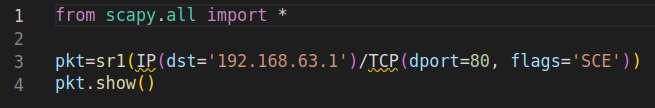
\includegraphics[width=\textwidth]{figures/congestione.png}
	\caption{Comando python per l'invio del pacchetto specifico}
	\label{congestione}
\end{figure}

\begin{table}[h]
	\centering
	\begin{tabular}{ l | c }
		\hline
		\rowcolor{blue!10} Windows 11 & 0
		\\
		\hline
		\rowcolor{red!10} Kali & 1
		\\
		\hline
		
	\end{tabular}
	\caption{ECN in risposta a specifico pacchetto}
	\label{tab:ECN}
\end{table}


\section{Livello 7: analisi protocollo HTTP}
Sebbene HTTP sia un protocollo a livello applicativo, esso consente ugualmente di ricavare alcune informazioni utili per l'OS fingerprinting: il campo \textit{user-agent}, infatti, contiene informazioni esplicite riguardanti il browser che si sta utilizzando e il sistema operativo in utilizzo. Questo tipo di situazione prende il nome di \textit{banner grabbing}.

A questo livello dello stack, si può inoltre tentare un fingerprinting che vada oltre l'individuazione del sistema operativo, ponendo come obiettivo quello di indovinare il tipo di applicativo in uso.
Questo è reso possibile dal fatto che HTTP è un protocollo di tipo testuale, pertanto non vi sono campi prefissati per ogni funzione. 
Ogni header contiene varie coppie, secondo lo schema:\\
\textbf{chiave:valore} 


Questo, a differenza dei protocolli analizzati precedentemente, permette un diverso ordine con le quali le coppie vengono elencate, essendo questo ininfluente per una corretta comunicazione. Analizzare l'ordinamento è molto importante se si vuole tentare di individuare, ad esempio, il tipo di server che sta rispondendo.






